\begin{filecontents*}[overwrite]{awe-references.bib}
@misc{blsoews2025,
  author={{U.S. Bureau of Labor Statistics}},
  title={National Employment and Wage Data by Occupation, May 2025},
  year={2026},
  howpublished={\url{https://www.bls.gov/news.release/ocwage.t01.htm}},
  note={Released May 15, 2026. Accessed October 25, 2026.}
}
@misc{blsoewsfaq,
  author={{U.S. Bureau of Labor Statistics}},
  title={Occupational Employment and Wage Statistics: Frequently Asked Questions},
  year={2026},
  howpublished={\url{https://www.bls.gov/oes/oes_ques.htm}},
  note={Accessed October 25, 2026.}
}
@misc{blsecec2026,
  author={{U.S. Bureau of Labor Statistics}},
  title={Employer Costs for Employee Compensation: Private Industry by Occupational Group, June 2026},
  year={2026},
  howpublished={\url{https://www.bls.gov/news.release/ecec.t04.htm}},
  note={Released September 9, 2026. Accessed October 25, 2026.}
}
@misc{onetprocurement,
  author={{National Center for O*NET Development}},
  title={Procurement Clerks, 43-3061.00},
  year={2026},
  howpublished={\url{https://www.onetonline.org/link/summary/43-3061.00}},
  note={Accessed October 25, 2026.}
}
@misc{onetwriters,
  author={{National Center for O*NET Development}},
  title={Technical Writers, 27-3042.00},
  year={2026},
  howpublished={\url{https://www.onetonline.org/link/summary/27-3042.00}},
  note={Accessed October 25, 2026.}
}
@misc{onetplanning,
  author={{National Center for O*NET Development}},
  title={Production, Planning, and Expediting Clerks, 43-5061.00},
  year={2026},
  howpublished={\url{https://www.onetonline.org/link/summary/43-5061.00}},
  note={Accessed October 25, 2026.}
}
@misc{onetprogrammers,
  author={{National Center for O*NET Development}},
  title={Computer Programmers, 15-1251.00},
  year={2026},
  howpublished={\url{https://www.onetonline.org/link/summary/15-1251.00}},
  note={Accessed October 25, 2026.}
}
@misc{openaisol2026,
  author={{OpenAI}},
  title={GPT-6.1 Sol Model: API Pricing},
  year={2026},
  howpublished={\url{https://developers.openai.com/api/docs/models/gpt-6.1-sol}},
  note={Standard short-context tariff. Accessed October 25, 2026.}
}
@misc{openaitools2026,
  author={{OpenAI}},
  title={OpenAI API Pricing},
  year={2026},
  howpublished={\url{https://developers.openai.com/api/docs/pricing}},
  note={Tool tariffs. Accessed October 25, 2026.}
}
@article{noyzhang2023,
  author={Noy, Shakked and Zhang, Whitney},
  title={Experimental Evidence on the Productivity Effects of Generative Artificial Intelligence},
  journal={Science},
  volume={381},
  number={6654},
  pages={187--192},
  year={2023},
  doi={10.1126/science.adh2586}
}
@misc{becker2025,
  author={Becker, Joel and Rush, Nate and Barnes, Elizabeth and Rein, David},
  title={Measuring the Impact of Early-2025 AI on Experienced Open-Source Developer Productivity},
  year={2025},
  eprint={2507.09089},
  archivePrefix={arXiv},
  howpublished={\url{https://arxiv.org/abs/2507.09089v2}},
  note={Version 2, July 25, 2025.}
}
@misc{metrupdate2026,
  author={Becker, Joel and Rush, Nate and Cunningham, Tom and Rein, David and Mahamud, Khalid},
  title={We Are Changing Our Developer Productivity Experiment Design},
  year={2026},
  howpublished={\url{https://metr.org/blog/2026-02-24-uplift-update/}},
  note={February 24, 2026. Accessed October 25, 2026.}
}

@misc{alphaevolve2025,
 author={Alexander Novikov and others},
 title={AlphaEvolve: A Coding Agent for Scientific and Algorithmic Discovery},
 year={2025},
 howpublished={\url{https://arxiv.org/abs/2506.13131}},
 note={Accessed October 25, 2026.}
}

@misc{criticgpt2024,
 author={Nat McAleese and others},
 title={LLM Critics Help Catch LLM Bugs},
 year={2024},
 howpublished={\url{https://arxiv.org/abs/2407.00215}},
 note={Accessed October 25, 2026.}
}

@misc{scipymilp,
 author={{SciPy developers}},
 title={scipy.optimize.milp: Mixed-Integer Linear Programming},
 year={2026},
 howpublished={\url{https://docs.scipy.org/doc/scipy/reference/generated/scipy.optimize.milp.html}},
 note={Accessed October 25, 2026.}
}

@misc{alphasource,
 author={{MONTREAL.AI}},
 title={AGI-Alpha-Agent-v0: Pinned Public Source},
 year={2026},
 howpublished={\url{https://github.com/MontrealAI/AGI-Alpha-Agent-v0/tree/a026e68413ab2e2d6086c758efc8abff723fdfe4}},
 note={Accessed October 25, 2026.}
}

@misc{managersource,
 author={{MONTREAL.AI}},
 title={AGIJobManager: Pinned Public Source},
 year={2026},
 howpublished={\url{https://github.com/MontrealAI/AGIJobManager/tree/5d5670df9dbbc79da115e0a44b71989f34df58c1}},
 note={Accessed October 25, 2026.}
}

@misc{jobssource,
 author={{MONTREAL.AI}},
 title={AGIJobsv0: Pinned Public Source},
 year={2026},
 howpublished={\url{https://github.com/MontrealAI/AGIJobsv0/tree/bc4abbd5c28f3672275b13300e40ea26c820b8ee}},
 note={Accessed October 25, 2026.}
}

@misc{fleetsource,
 author={{MONTREAL.AI}},
 title={AGI-Fleet-Linux: Pinned Public Source},
 year={2026},
 howpublished={\url{https://github.com/MontrealAI/AGI-Fleet-Linux/tree/45759fb096faf8988f58ae5ea71248d0f35a97c7}},
 note={Accessed October 25, 2026.}
}

@misc{managercontract,
 author={{MONTREAL.AI}},
 title={contracts/AGIJobManager.sol: Inspected Contract Source},
 year={2026},
 howpublished={\url{https://github.com/MontrealAI/AGIJobManager/blob/5d5670df9dbbc79da115e0a44b71989f34df58c1/contracts/AGIJobManager.sol}},
 note={Accessed October 25, 2026.}
}

@misc{ascensioncontract,
 author={{MONTREAL.AI}},
 title={contracts/ascension/AscensionJobMarket.sol: Inspected Contract Source},
 year={2026},
 howpublished={\url{https://github.com/MontrealAI/AGI-Alpha-Agent-v0/blob/a026e68413ab2e2d6086c758efc8abff723fdfe4/contracts/ascension/AscensionJobMarket.sol}},
 note={Accessed October 25, 2026.}
}

@misc{markcontract,
 author={{MONTREAL.AI}},
 title={contracts/ascension/AscensionMark.sol: Inspected Contract Source},
 year={2026},
 howpublished={\url{https://github.com/MontrealAI/AGI-Alpha-Agent-v0/blob/a026e68413ab2e2d6086c758efc8abff723fdfe4/contracts/ascension/AscensionMark.sol}},
 note={Accessed October 25, 2026.}
}

@misc{feepoolcontract,
 author={{MONTREAL.AI}},
 title={contracts/v2/FeePool.sol: Inspected Contract Source},
 year={2026},
 howpublished={\url{https://github.com/MontrealAI/AGIJobsv0/blob/bc4abbd5c28f3672275b13300e40ea26c820b8ee/contracts/v2/FeePool.sol}},
 note={Accessed October 25, 2026.}
}

\end{filecontents*}
\begin{filecontents*}[overwrite]{awe-costs.tex}
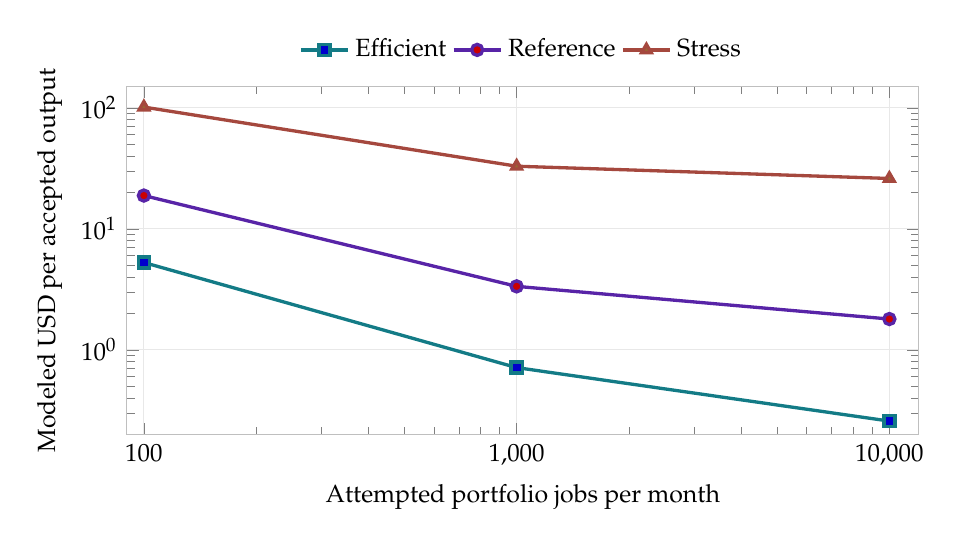
\begin{tikzpicture}
\begin{axis}[width=0.96\linewidth,height=6.0cm,xmode=log,ymode=log,xmin=90,xmax=12000,ymin=0.2,ymax=150,xtick={100,1000,10000},xticklabels={100,{1,000},{10,000}},xlabel={Attempted portfolio jobs per month},ylabel={Modeled USD per accepted output},grid=major,grid style={gray!18},axis line style={gray!50},tick label style={font=\small},label style={font=\small},legend style={at={(0.5,1.04)},anchor=south,legend columns=3,draw=none,font=\small}]
\addplot+[color=teal,mark=square*,line width=1.2pt] coordinates {(100,5.274527049671836) (1000,0.714168841321525) (10000,0.25813302048649384)};
\addlegendentry{Efficient}
\addplot+[color=purple,mark=*,line width=1.2pt] coordinates {(100,18.86010657077143) (1000,3.350760657077142) (10000,1.799826065707714)};
\addlegendentry{Reference}
\addplot+[color=coral,mark=triangle*,line width=1.2pt] coordinates {(100,101.54324699873555) (1000,32.96083640555918) (10000,26.102595346241536)};
\addlegendentry{Stress}
\end{axis}\end{tikzpicture}
\end{filecontents*}
\begin{filecontents*}[overwrite]{awe-transfer.tex}
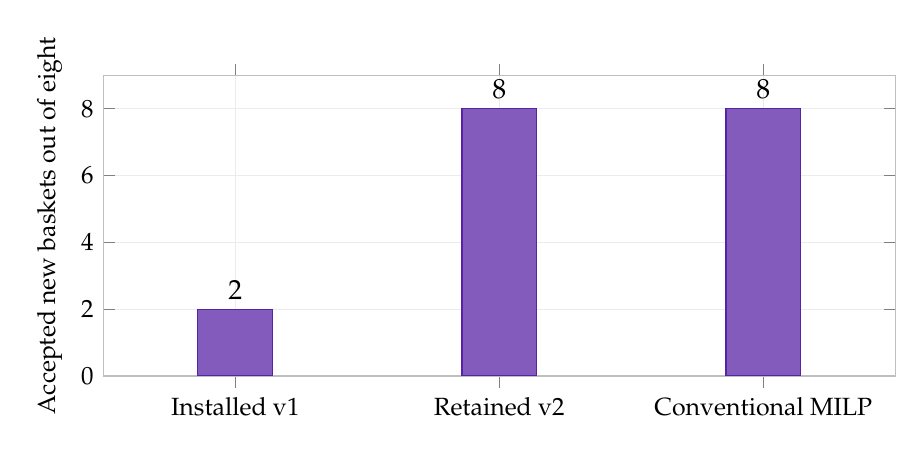
\begin{tikzpicture}
\begin{axis}[width=0.96\linewidth,height=5.4cm,ybar,bar width=27pt,ymin=0,ymax=9,ytick={0,2,4,6,8},symbolic x coords={Installed v1,Retained v2,Conventional MILP},xtick=data,ylabel={Accepted new baskets out of eight},nodes near coords,point meta=y,grid=major,grid style={gray!15},axis line style={gray!50},tick label style={font=\small},label style={font=\small},enlarge x limits=0.25]
\addplot[fill=purple!75,draw=purple] coordinates {(Installed v1,2) (Retained v2,8) (Conventional MILP,8)};
\end{axis}\end{tikzpicture}
\end{filecontents*}
\begin{filecontents*}[overwrite]{awe-cash.tex}
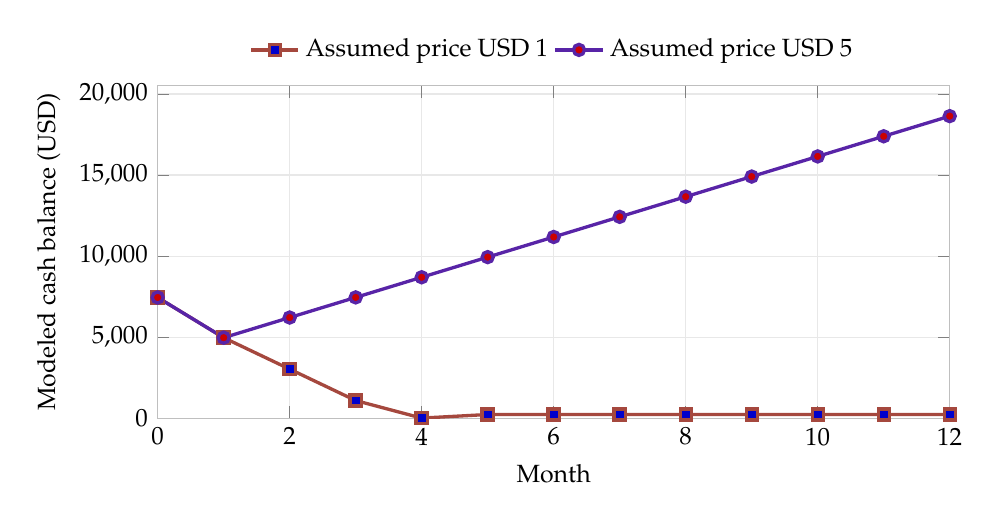
\begin{tikzpicture}
\begin{axis}[width=0.96\linewidth,height=5.8cm,xmin=0,xmax=12,ymin=0,xlabel={Month},ylabel={Modeled cash balance (USD)},xtick={0,2,4,6,8,10,12},scaled y ticks=false,y tick label style={/pgf/number format/fixed,/pgf/number format/precision=0},grid=major,grid style={gray!18},axis line style={gray!50},tick label style={font=\small},label style={font=\small},legend style={at={(0.5,1.04)},anchor=south,legend columns=2,draw=none,font=\small}]
\addplot+[color=coral,mark=square*,line width=1.2pt] coordinates {(0,7444.507222244016) (1,4963.004814829344) (2,3023.2304074146714) (3,1083.4559999999992) (4,0.6921700853270067) (5,222.258922085327) (6,222.258922085327) (7,222.258922085327) (8,222.258922085327) (9,222.258922085327) (10,222.258922085327) (11,222.258922085327) (12,222.258922085327)};
\addlegendentry{Assumed price USD 1}
\addplot+[color=purple,mark=*,line width=1.2pt] coordinates {(0,7444.507222244016) (1,4963.004814829344) (2,6205.882407414671) (3,7448.759999999999) (4,8691.637592585328) (5,9934.515185170658) (6,11177.392777755987) (7,12420.270370341317) (8,13663.147962926647) (9,14906.025555511977) (10,16148.903148097306) (11,17391.780740682636) (12,18634.658333267966)};
\addlegendentry{Assumed price USD 5}
\end{axis}\end{tikzpicture}
\end{filecontents*}
\documentclass[11pt,letterpaper]{article}
\usepackage[T1]{fontenc}
\usepackage[utf8]{inputenc}
\usepackage{mathpazo}
\usepackage[scaled=0.92]{helvet}
\usepackage{microtype}
\usepackage[margin=0.85in,headheight=15pt]{geometry}
\usepackage{amsmath,amssymb,booktabs,tabularx,longtable,array,enumitem}
\usepackage[table]{xcolor}
\usepackage{graphicx,tikz,pgfplots,tcolorbox,fancyhdr,seqsplit,placeins}
\usetikzlibrary{arrows.meta,positioning,calc}
\pgfplotsset{compat=1.18}
\usepackage[numbers,sort&compress]{natbib}
\usepackage{xurl}
\usepackage[colorlinks=true,linkcolor=purple,citecolor=purple,urlcolor=teal,bookmarksopen=true]{hyperref}
\definecolor{purple}{HTML}{5824A7}
\definecolor{deep}{HTML}{180D31}
\definecolor{lavender}{HTML}{F4F0FC}
\definecolor{teal}{HTML}{137B86}
\definecolor{coral}{HTML}{A5483E}
\definecolor{ink}{HTML}{202333}
\hypersetup{pdftitle={AGI ALPHA FLYWHEEL: The Autonomous Work Economy},pdfauthor={Vincent Boucher - MONTREAL.AI},pdfsubject={AWE-2026-01: bounded delivery, capability transfer, and conditional economics},pdfkeywords={AGI ALPHA, autonomous work, unit economics, capability transfer, reproducibility}}
\urlstyle{same}
\setlength{\parindent}{0pt}
\setlength{\parskip}{5.3pt}
\setlength{\tabcolsep}{5pt}
\renewcommand{\arraystretch}{1.17}
\setlist{nosep,leftmargin=1.5em}
\pagestyle{fancy}\fancyhf{}
\fancyhead[L]{\sffamily\scriptsize\color{purple}AGI ALPHA FLYWHEEL}
\fancyhead[R]{\sffamily\scriptsize\color{gray}AWE-2026-01\quad |\quad Research edition 1.0}
\fancyfoot[L]{\sffamily\scriptsize\color{gray}The Autonomous Work Economy}
\fancyfoot[R]{\sffamily\small\thepage}
\renewcommand{\headrulewidth}{0.3pt}
\color{ink}
\raggedbottom
\setlength{\emergencystretch}{1.5em}
\renewcommand{\topfraction}{0.9}
\renewcommand{\textfraction}{0.05}
\renewcommand{\floatpagefraction}{0.75}
\makeatletter\setlength{\@fptop}{0pt}\setlength{\@fpsep}{15pt}\setlength{\@fpbot}{0pt plus 1fil}\makeatother
\begin{document}
\hypersetup{pageanchor=false}
\begin{titlepage}
\begin{tikzpicture}[remember picture,overlay]
\fill[deep] (current page.south west) rectangle (current page.north east);
\fill[purple!50!deep] ($(current page.north east)+(-1.0,-1.8)$) circle (4.7cm);
\draw[white!15,line width=0.6pt] ($(current page.north east)+(-2.6,-2.4)$) circle (5.7cm);
\draw[white!12,line width=0.6pt] ($(current page.north east)+(-2.6,-2.4)$) circle (7.2cm);
\foreach \x/\y/\r in {1/1/.025,3/2/.018,5/1.4/.025,8/1/.02,12/2/.025,16/1/.025,2/6/.018,17/8/.02,16/12/.025,2/16/.02,18/19/.02,4/23/.02,13/24/.02}{\fill[white!70] ($(current page.north west)+(\x,-\y)$) circle (\r cm);}
\end{tikzpicture}
\color{white}\sffamily
\vspace*{0.6cm}
{\small\bfseries MONTREAL.AI\hfill RESEARCH EDITION 1.0}\par
\vspace{1.4cm}
{\large\color{white!75}AGI ALPHA FLYWHEEL\quad $\infty$}\par
\vspace{0.4cm}
{\fontsize{37}{41}\selectfont\bfseries THE AUTONOMOUS\\WORK ECONOMY}\par
\vspace{0.7cm}
{\Large From Useful Outcomes to\\Expanding Productive Capability}\par
\vspace{0.8cm}
\rule{2.0cm}{1.0pt}\par
\vspace{0.3cm}
{\large SUCCESSOR $\Omega$ HARNESS}\par
{\small\bfseries ACTIVATE. EVOLVE. SCALE.}\par
\vspace{0.3cm}
{\small Powered by TRANSFORMATIONAL INTELLIGENCE $\infty$\\and the applicable \$AGIALPHA utility.}\par
\vfill
\begin{minipage}{0.94\linewidth}
{\large\bfseries Useful work. Inspectable evidence. Earned growth.}\par
\vspace{0.35cm}
{\normalsize An executable study of bounded digital work, retained capabilities,\\conditional unit economics and cash-constrained reinvestment.}\par
\vspace{0.5cm}
{\small 24 primary structural cases\quad $\cdot$\quad 8 separate transfer probes}\par
{\small Observed local delivery\quad $\cdot$\quad Modeled enterprise economics}\par
\vspace{0.7cm}
{\small Vincent Boucher\quad $\cdot$\quad MONTREAL.AI\\25 October 2026\quad |\quad Study AWE-2026-01}
\end{minipage}
\vspace*{0.3cm}
\end{titlepage}
\hypersetup{pageanchor=true}
\setcounter{page}{1}
\begin{center}{\Large\bfseries AGI ALPHA FLYWHEEL: The Autonomous Work Economy}\par
\small Vincent Boucher $\cdot$ MONTREAL.AI\quad |\quad 25 October 2026
\end{center}
\section*{Abstract}
Automated digital work can produce immediate customer value without first proving universal capability or self-acceleration. We study the connection between bounded useful delivery, complete operating cost, retained executable capability, and reinvestment. A frozen 24-case engineering census executes four artifact families through the existing AGI ALPHA Workbench: 16 supported cases deliver contract-accepted packets, and eight intended negative cases are refused. Separate algorithms verify acceptance; a conventional MILP confirms every quote optimum. An executable capability is retained and reused, an incorrect greedy candidate is rejected, and an allowlisted successor is composed. On eight separately frozen new transfer baskets, the successor and conventional MILP solve all eight; the initial capsule supports two and refuses six. This establishes bounded transfer and installed-workflow enablement, not novel algorithm discovery. Actual full enterprise costs remain unknown. Price-calibrated economic sensitivities model missing operations, failures, shared upkeep and residual attention. At an assumed 1,000 attempted monthly jobs, reference model-extension full cost is USD 3.351 per accepted result; a separately frozen automatic-upkeep configuration yields USD 2.817. Neither is an observed cost. Human comparisons use source-backed break-even time because matched non-AI task durations are unavailable. Cash-constrained simulations distinguish external funding, collected proceeds, reserves and financeable investment; no candidate is economically admitted without demonstrated monetized benefit. The study delivers an offline bilingual working demonstration, source, protocols, raw evidence and reproducible analysis. Authenticated enterprise execution, realized self-financing and self-acceleration remain unestablished.

\section*{R\'esum\'e}
Cette \'etude relie des livrables utiles, leur co\^ut complet, la r\'eutilisation de capacit\'es ex\'ecutables et le financement de nouvelles capacit\'es. Le protocole principal comprend 24 cas structur\'es: 16 livrables sont accept\'es selon leur contrat et huit entr\'ees hors p\'erim\`etre sont refus\'ees. Une exp\'erience distincte porte sur huit nouveaux paniers de devis. Les comparaisons \`a la main-d'\oe uvre reposent sur des seuils de rentabilit\'e conditionnels, sans dur\'ees humaines invent\'ees. Les co\^uts et encaissements de l'entreprise sont mod\'elis\'es; aucun paiement client ni autofinancement r\'ealis\'e n'est observ\'e. La d\'emonstration bilingue produit un r\'esultat local inspectable. L'auto-acc\'el\'eration n'est pas \'etablie.

\begin{tcolorbox}[colback=lavender,colframe=purple,title={Reading the evidence}]
\textbf{Observed} denotes actual local execution or an inspected artifact. \textbf{Sourced} denotes external published data. \textbf{Estimated/assumed} denotes a declared model input. \textbf{Unknown} remains unknown. \textbf{NOT RUN} denotes an unperformed operational test. A recorded artifact, a simulation and a fresh execution are never interchangeable.
\end{tcolorbox}
\clearpage
\tableofcontents
\clearpage
\section{Research question and contribution}

An automated worker becomes economically useful when it produces an outcome that a customer can use at a justified total cost. Retaining a useful method can expand that worker's productive capacity. Financing that expansion, however, requires collected proceeds, affordable obligations, and an investment whose incremental benefits exceed its complete costs. These are separate propositions. A low computation bill cannot establish all of them.

This study asks: \emph{Can an automated AGI ALPHA enterprise deliver valuable digital work at a compelling total cost relative to competent traditional human work, and can resources generated by that activity support additional productive capabilities whose benefits justify construction and upkeep?} The empirical answer is deliberately bounded. We executed local artifact workflows through the existing AGI ALPHA Workbench, evaluated reusable capability composition, and constructed a prospective economic model for missing production operations. We did not execute an authenticated autonomous enterprise or observe sales.

\paragraph{The original contribution.} AWE-2026-01 contributes an inspectable connection between four objects often conflated: a usable artifact, a retained executable capability, an economically available dollar, and an admissible capability investment. The contribution consists of (i) a frozen engineering census across four bounded work families; (ii) a connected retention, reuse, rejection and successor sequence, supplemented by new post-freeze transfer inputs; (iii) independent-algorithm acceptance and fault checks; (iv) a price-calibrated, assumption-explicit model of full delivery costs and cash-constrained reinvestment; and (v) a bilingual, offline demonstration that produces a fresh quote-comparison packet. The optimization methods are conventional. We make no claim of a new general-purpose solver, superior model, or autonomous scientific discovery.

\paragraph{Strategic deployment as the unit of improvement.} The relevant object is not merely a previous answer. It can be a normalizer, a solver-selection rule, a regression case, a source-evidence representation, or a repair procedure. Such objects change how available intelligence and computation are deployed. A higher-order improvement would improve how these methods are discovered. We distinguish that objective from the bounded composition actually observed here. Its search kernels and admissible templates were externally authored; improvement of their discovery process was not demonstrated.

\paragraph{Related evidence.} AlphaEvolve combines model proposals with automated evaluation to improve algorithms \cite{alphaevolve2025}; CriticGPT investigates evidence-producing criticism of generated code \cite{criticgpt2024}. These support studying proposal and verification mechanisms, but their results do not transfer to this implementation. Task-performance experiments in writing and software development also differ in workers, tools, tasks, and oversight responsibilities \cite{noyzhang2023,becker2025,metrupdate2026}. They motivate task-specific measurement. We do not import a productivity ratio or human duration from a different setting.

\section{Actual foundations and execution boundary}

The study inspected all four project foundations at immutable source identities (Appendix~\ref{app:pins}). The existing Alpha API exposes \texttt{createWorkbench} with planning, execution and export-inspection operations: \texttt{plan}, \texttt{run} and \texttt{inspectPack}. Seven upstream JavaScript modules and their Apache license were preserved byte-for-byte. A separate source audit retrieved 35 public files and verified each against its Git blob identity. Repository metadata and historical deployment records were inspected; neither source inspection nor a published release label is a new production qualification \cite{alphasource,managersource,jobssource,fleetsource}.

Three study adapters use that extension seam: quotes, structured evidence briefs, and dependency and resource plans. The software-maintenance family calls the native finite-grammar reliability and documentation handlers. The original runtime compiles a typed job plan, binds inputs and source identities, executes the chosen specialist, checkpoints, validates artifacts, and produces an integrity-bound export. No upstream runtime source was changed. Actual runtime records retain \texttt{PUBLIC\_LOCAL\_EXECUTION}, \texttt{HOLD}, null model/provider identities, unknown compute and human costs, and \texttt{NOT\_CONNECTED} settlement.

\begin{tcolorbox}[colback=lavender,colframe=purple,title={The scope of execution}]
Observed: local deterministic artifact production through the pinned AGI ALPHA Workbench.\par
Not run: authenticated browser-to-approved-executor operation, model-mediated intake and reasoning, Fleet commissioning, live payments, fresh chain verification, and a new human task trial.\par
The research assistants used models to author and inspect this study. Their authoring usage was not metered as production execution and is not reported as zero.
\end{tcolorbox}

The project's seven-stage sequence has a concrete interpretation here (Table~\ref{tab:stages}). It is a mapping from decisions to artifacts, not evidence that seven independent model agents executed. Stages share data and are combined when an extra pass would provide no verified benefit. The full operating map also includes input preparation, verification, correction, packaging, reporting, and recovery. Every missing production activity is retained as an unknown or explicit economic assumption.

\begin{table}[htbp]\centering\small
\caption{Operational meaning of the seven stages in the executed route.}\label{tab:stages}
\begin{tabularx}{\linewidth}{@{}lXX@{}}\toprule
Stage & Useful artifact or decision & Evidence boundary\\\midrule
Identify & Bounded contract, permitted input classification, scope and deadline & User chooses purpose and rights; no inferred permission.\\
Out-Learn & Parsed offers or supplied source register & Explicit rates and source metadata; no live model learning.\\
Out-Think & Constraint model and candidate methods & Finite deterministic reasoning and known algorithms.\\
Out-Design & Report/CSV/JSON schema and acceptance checks & Original adapters; supplied acceptance contracts.\\
Out-Strategise & Select a fixed-shipping-aware specialist; preserve MILP & No requirement to adopt a new method.\\
Out-Execute & Run, checkpoint, verify, package and export & Actual source-bound Workbench invocations.\\
Out-Evolve & Retain capsule and regression; compose bounded successor & Actual executable reuse; no novel algorithm discovery.\\\bottomrule
\end{tabularx}
\end{table}

\section{Prospective design and acceptance}

\subsection{Portfolio, sample size and unsupported work}

The primary protocol fixed 24 structural cases before confirmation: six per family, with four intended supported deliveries and two intentionally invalid or unsupported cases. The size was chosen as an engineering census spanning named constraints and refusal paths within available resources. It is not a powered sample of a job population. Cases share authored grammars; the authors were not blinded to the generators. Repeated timings, alternative methods, injected faults and the later transfer extension do not increase the primary count or occupational breadth.

The selection favors recognizable deliverables with checkable acceptance and permitted inputs. A quote packet organizes quantities, pack sizes, currency ratios, shipping and delivery limits. A brief preserves facts and source qualifications. A plan resolves dependencies and resource collisions. A maintenance packet preserves originals and supplies a correction or verified example. None of these demonstrations establishes an entire occupation's automation. General repository maintenance, autonomous web research, original long-form writing, private records, customer credentials, physical operations and external transactions are outside the tested scope.

The workflow inventory and input hashes were frozen locally before confirmation, as were the implementation and economic assumptions before their corresponding calculations. These are timestamped local freezes, not registration with an external preregistration service. Original results and all later amendments remain separately identified. The production cost model was formulated with knowledge of the bounded design; it does not masquerade as an empirical cost measurement or a prediction confirmed by the same fixture outcomes.

\subsection{Acceptance contracts}

For quotes, acceptance requires one offer per item, sufficient delivered quantities, valid supplied conversion ratios, the delivery deadline, exact half-up integer-currency arithmetic, fixed shipping paid once per used supplier, and agreement with an independently implemented mixed-integer linear program. The conventional SciPy/HiGHS solver remains available \cite{scipymilp}. Taxes, split purchases, uncertain inventory, discounts and qualitative supplier preferences are excluded. A result is conditional on complete and correct inputs.

For briefs, every requested factual record, source URL, period, geography, coverage and qualification must be preserved. This is offline transformation of a researched register, not a fresh factual investigation. For plans, acceptance checks full task coverage, predecessor order, duration arithmetic, resource non-overlap and the declared deadline. The list scheduler is not claimed globally optimal; its deadline refusal does not prove that all other scheduling methods would fail. For software, acceptance checks the finite range grammar or named URI/UTF-8 operation against separate Python logic while preserving originals and a usable patch or example packet.

\subsection{Verification, criticism and independence}

The creator produces a packet. A challenger supplies an executable constraint violation or an altered artifact. An adjudicator checks the claim against the source input and declared contract. Twelve deliberate semantic mutations were evaluated separately; no unsupported criticism was allowed to trigger a change. The fixed-shipping greedy counterexample became a retained regression. These roles are implemented algorithms, not an assertion that agreement among models proves correctness.

Python normalization, acceptance logic and the MILP incumbent were separate from the JavaScript candidate execution. Economics and source audits were separately implemented by sibling research agents. They share a supervising session, model family and accessible artifacts. This independence is computational and organizational within one team; it is not external, blinded, adversarial peer review. Common specifications can still contain common errors. Hashes establish identity and integrity, not truth.

The scrutiny budget is bounded: a fixed conformance census, named mutations, deterministic limits, and explicit termination. Five actual control checks exercise cancellation, recovery by a fresh invocation, export/import integrity, tamper rejection and input-classification enforcement. Nothing in an imported record authorizes external execution. Failed or uncertain work must be reconciled rather than silently accepted.

\section{Observed useful delivery}

\begin{table}[htbp]\centering\small
\caption{Primary frozen census. Acceptance is by the study contract, not an observed customer purchase.}\label{tab:primary}
\begin{tabularx}{\linewidth}{@{}Xrrr@{}}\toprule
Family & Cases & Accepted artifacts & Expected refusals\\\midrule
Complete quote comparison & 6 & 4 & 2\\
Source-register evidence brief & 6 & 4 & 2\\
Dependency/resource plan & 6 & 4 & 2\\
Finite software maintenance & 6 & 4 & 2\\\midrule
Total & 24 & 16 & 8\\\bottomrule
\end{tabularx}
\end{table}

All 16 supported cases produced contract-accepted artifacts; all eight negative cases produced the intended refusals. There were no unexpected primary confirmation failures. Refusal is useful containment but is not a delivered outcome and is never counted as an accepted sale. The batch generated 111,669 artifact bytes in 626.53 ms wall time in the recorded environment. That is a small local batch measurement, excluding preparation, authoring, research engineering, customer assessment and production operation. Individual accepted family medians were approximately 58, 32, 29 and 25 ms for quotes, briefs, plans and software respectively. Runtime provider and settlement calls were zero for this route.

All four quote optima matched the separate MILP implementation. The 12 known semantic mutations were detected, with no false alarm on the 16 supported originals. This is a diagnostic result on a small deliberately constructed fault set. It does not estimate production sensitivity, specificity, defect prevalence or the chance of an undiscovered serious error. Review cost is included as local verifier time in raw records and as assumed production work in the economic model; it is not presumed free.

\subsection{Flagship: an inspectable equipment quote packet}

Case Q2 compares six requested items against 24 offers from four synthetic suppliers. It includes three currencies, explicit conversion ratios, pack rounding, a six-day deadline and fixed supplier shipping. The output is a recommended cart, a line-item CSV, a written decision packet and a JSON audit record. It selects a total of \textbf{USD 520.12}, comprising USD 493.90 in lines and USD 26.22 in shipping (Table~\ref{tab:cart}). This is an optimization result on synthetic prices, not an actual supplier quote, customer saving or procurement action.

\begin{table}[htbp]\centering\small
\caption{Q2 recommended basket. Required and delivered quantities differ because whole packs are purchased in the model.}\label{tab:cart}
\begin{tabular}{@{}llrrrr@{}}\toprule
Item & Supplier & Required & Delivered & Packs & Line USD\\\midrule
Monitor & Delta & 11 & 15 & 3 & 102.72\\
Dock & Delta & 2 & 5 & 1 & 38.58\\
Keyboard & Delta & 13 & 15 & 3 & 101.97\\
Desk lamp & Cedar & 2 & 5 & 1 & 55.68\\
USB hub & Cedar & 7 & 10 & 2 & 88.45\\
Cable pack & Aster & 10 & 10 & 2 & 106.50\\\midrule
\multicolumn{5}{l}{Line subtotal} & 493.90\\
\multicolumn{5}{l}{Shipping: Aster 13.77 + Cedar 8.21 + Delta 4.24} & 26.22\\
\multicolumn{5}{l}{Complete modeled basket} & \textbf{520.12}\\\bottomrule
\end{tabular}
\end{table}

The nontechnical value proposition is concrete: provide a permitted offer table, obtain a complete eligible basket, inspect the arithmetic and assumptions, and export a result usable in a purchasing decision. The software does not purchase. Whether a customer would pay for this packet, and how much time it saves relative to their ordinary spreadsheet process, remain unmeasured. The bilingual demonstration accepts fresh user-supplied permitted inputs under the same bounded contract; that makes the artifact useful beyond replaying the example while preserving its limits.

\section{Capability retention, transfer and construction}

\subsection{A connected sequence with a rejected candidate}

The initial capability is an executable capsule using exact normalization and a bounded exhaustive cart solver. A development mission produces an inspectable result, and the emitted capsule is invoked on Q1. A deliberately simple per-item greedy candidate is then constructed and challenged. It selects two individually cheap lines but pays shipping twice, giving USD 22.00 where a valid USD 13.00 cart exists. The candidate is rejected and the counterexample retained. Rejecting that proposal is part of the result, not a failed narrative that should be removed.

The changed Q2 requirement introduces packs and nonidentity currency ratios. The original capsule refuses its declared scope. A successor capsule is emitted through an allowlisted composition of the already-authored normalizer and an exact vendor-subset specialist. It is actually invoked on Q2 and Q4 and its outputs checked. Q4 contains fourteen items and four offers per item: naive exhaustive enumeration has $4^{14}=268{,}435{,}456$ combinations, while the vendor-subset procedure examines $2^4-1=15$ subsets. A conventional MILP also solves it. Enablement is therefore relative to the installed v1 constraints, not a capability beyond established optimization tools.

For each nonempty supplier subset, the procedure selects the cheapest eligible line per item and evaluates the cost including shipping for suppliers actually used. With nonnegative fixed shipping and independent item choices, examining every subset includes the supplier set of any globally optimal cart. Choosing cheaper lines within that set cannot increase its line cost or introduce a supplier outside it. Evaluating the actual used set therefore includes a cart with objective no worse than that optimum. This explains exactness under the declared contract. Discounts, capacities, split purchases or other coupling would invalidate the argument and require a new solver/contract.

\subsection{A separate genuinely new input extension}

The original capsule sequence reuses Q2 and Q4 after the primary results are known. It establishes execution and dependency, but it is not unseen confirmation of a newly discovered algorithm. To strengthen the transfer claim, a separate eight-case extension froze the unchanged capsules, generator, acceptance code and analysis before generating its new inputs. Seeds 7001--7008 span 4--18 items, 3--5 suppliers, pack/currency changes and larger search spaces. The extension was designed after the primary results and is labeled accordingly.

The successor produces eight of eight independently optimal packets on these new baskets. The initial capsule supports two; it refuses two because of its 50,000-combination limit and four because of pack/currency scope. The retained MILP supports all eight (Figure~\ref{fig:transfer}). These are eight structural transfer probes within one family, not eight new work families or a population success rate.

\begin{figure}[htbp]\centering\input{awe-transfer.tex}
\caption{Separate post-capsule transfer extension. All methods receive identical new inputs. The successor expands the installed capsule's supported set, while the conventional MILP remains fully capable.}\label{fig:transfer}
\end{figure}

The first extension reporting script raised an error while formatting a null parent result after all eight Workbench outputs had been produced. The original source, freeze, inputs and results were preserved. A separately versioned null-handling correction and completion audit evaluated every original output without changing the solver or acceptance rule. Appendix~\ref{app:amendments} records the failure. This amendment is not retroactively part of the original freeze.

\subsection{Technical usefulness does not force economic promotion}

The capsule has applicability bounds, exact source identities, retained regressions and a rollback path to v1 or the conventional incumbent. Its construction event is measured file emission and invocation. The kernels, templates and research engineering are external resources with unknown original costs. Emission milliseconds cannot replace those costs.

Nine paired timing repetitions after warm-up on each of the four original quote cases show lower median solver latency for the subset method than the MILP, with mean savings of 1.476 ms. These timings exclude process startup, Workbench packaging, upkeep and engineering. At a whole-session price, both fit in the same session and the modeled bill difference is zero. Even continuous prorating at USD 0.09/hour yields only about $3.69\times10^{-8}$ dollars per call. Latency alone does not justify an assumed eight-hour construction budget at the studied volumes. The value of newly supported work may be larger, but demand and monetized benefit have not been measured. \textbf{Economic production promotion remains HOLD.}

\section{Economics: full costs and fair comparison}\label{sec:economics}






\subsection{Evidence boundary and comparison}

The economic finding is conditional: bounded delivery is observed, but its full
enterprise cost and commercial advantage are not. The local workflow records
execution time, artifacts, checks, and zero runtime provider or settlement calls.
Host charges, assistant authoring, development attention, production exceptions,
customer demand, and collections remain unmetered. Unknown is not zero. The
authenticated model enterprise is \texttt{NOT RUN}; none of the monetary totals
below is an observed invoice or customer payment.

We distinguish two prospective deployments. \emph{Hosted tool delivery} prices
the deterministic contracts that executed locally. \emph{Model extension} adds
proposed semantic intake, explanation, and independent checking calls. Those
stages have not executed, and their quality and usage are uncalibrated. Both
routes include delivery operations and shared upkeep; neither assumes a permanent
manual reviewer for every job. The efficient, reference, and stress settings are
explicit sensitivities, not forecasts or confidence bounds. Protocols and
parameters were frozen before their corresponding calculations; later liquidity
and upkeep amendments preserve earlier versions.

The primary comparator is competent human work using ordinary non-AI tools.
O*NET supports the match between the bounded contracts and procurement clerks,
technical writers, planning clerks, and programmers
\cite{onetprocurement,onetwriters,onetplanning,onetprogrammers}. It does not
establish the fraction of an occupation automated. We found no matched human
timing evidence for these exact deliverables, revisions, and acceptance duties.
Professional-writing and developer studies concern different tasks and tool
vintages; they supply context, not transferable durations
\cite{noyzhang2023,becker2025,metrupdate2026}. Wage surveys also do not establish
workers' AI usage. We therefore report break-even human times without claiming
measured savings or equivalent human quality.

\begin{table}[tbp]
\centering\small
\caption{U.S. occupational neighbors and annual wage-equivalent at an assumed 1,800 hours.}
\label{tab:ec-labor}
\begin{tabular}{llrrrr}
\toprule
Occupation & SOC & Jobs & Mean/h & Median/h & USD bn \\
\midrule
Procurement clerks & 43-3061 & 55,810 & 25.18 & 24.32 & 2.530 \\
Technical writers & 27-3042 & 45,500 & 46.62 & 43.46 & 3.818 \\
Planning clerks & 43-5061 & 390,160 & 29.88 & 28.68 & 20.984 \\
Computer programmers & 15-1251 & 92,230 & 50.56 & 48.26 & 8.394 \\
\bottomrule
\end{tabular}
\par\smallskip\begin{minipage}{0.97\linewidth}\footnotesize BLS May 2025 OEWS, released May 2026; hourly wages are USD and exclude nonwage benefits \cite{blsoews2025,blsoewsfaq}. Employment includes full- and part-time wage/salary jobs and excludes self-employment. The last column is employment $\times$ mean hourly wage $\times$ assumed annual hours; it is not observed payroll or GDP.
\end{minipage}
\end{table}


All monetary values are nominal USD. BLS May 2025 median hourly wages determine
the wage-only comparator; employment and mean wages determine the market
calculation \cite{blsoews2025}. An additional employer-cost approximation applies
June 2026 ECEC total-compensation/wage ratios of $73.69/50.98$ for professional
occupations and $36.73/25.22$ for office occupations \cite{blsecec2026}. These
broad groups and mixed vintages do not constitute occupation-specific employer
cost observations. Benefits already in these ratios must not be added again.
Facilities, subscriptions, and service-provider markup are excluded from that
human proxy. Support and customer attention use $w_s=46.89$ dollars/hour;
development uses the software-developer median of $65.38$ multiplied by
$73.69/50.98$, giving $w_d=94.50475$ dollars/hour. Both are declared proxies.

\subsection{Complete cost-to-outcome accounting}

Let $N$ denote jobs attempted at least once per month, excluding extra
computational retry passes, and let $f$ index a workflow family. One full retry
is allowed. In a normal month its probability is $r$, final acceptance is $p$,
and a common adverse month occurs with probability $q$. The adverse state adds
retry probability $d$ and retains fraction $k$ of normal acceptance. Define
\begin{align}
 a&=1+(1-q)r+q\min(1,r+d), &
 \bar p&=p\{(1-q)+qk\}. \label{eq:ec-acceptance}
\end{align}
Thus expected accepted volume is $N\bar p$, while expected computational passes
are $Na$. Production probabilities are assumptions, not the fraction of
confirmation fixtures that passed. A common shock affects the whole month;
it is not treated as independent noise on each job.

The cost of one computational pass is
\begin{equation}
 b_f=\frac{\alpha I_f+\beta O_f}{10^6}+\gamma W_f+\rho K_f,
 \label{eq:ec-pass}
\end{equation}
where $I_f,O_f$ are proposed input and billable output tokens (including
reasoning), $W_f$ search calls, and $K_f$ hosted sessions. Retrieved source text
is included in the proposed input budget. Published standard short-context
GPT-6.1 Sol tariffs, retrieved October 25, 2026, are $\alpha=2$ and $\beta=10$
dollars/million tokens \cite{openaisol2026}; search is $\gamma=0.01$ dollars/call
\cite{openaitools2026}. We assume a dedicated 1GB, 20-minute session at
$\rho=0.03$ dollars. Eligible sessions can have shorter billing increments;
the full-session route is an explicit conservative allowance, not a charge
inferred from local milliseconds. No caching discounts are assumed. In the
tool route, model tokens and search calls are zero. Reference extension
input/output budgets are 8,000/2,500 for quotes, 18,000/4,200 for briefs,
8,500/3,000 for plans, and 40,000/10,500 for source repair. Budgets are estimated
from proposed stages, not metered calls.

Let disjoint normal and rare exception categories have probabilities $u_n,u_r$
and handling minutes $t_n,t_r$. Their expected human expense per attempted job
is $e=w_s(u_nt_n+u_rt_r)/60$. Shared monthly expense is
$F=L+w_dh_m+w_sh_a+qw_dh_c$, covering platform/archive allowance $L$,
maintenance hours $h_m$, administration hours $h_a$, and adverse-month recovery
hours $h_c$. One-time shared setup is $D=w_dh_0$, allocated over $H=12$ months.
The cumulative cost tiers per accepted result are
\begin{align}
 C_f^{\mathrm{marg}}&=\frac{ab_f}{\bar p}, \label{eq:ec-marginal}\\
 C_f^{\mathrm{rec}}&=\frac{ab_f+e+F/N}{\bar p}, \label{eq:ec-recurring}\\
 C_f^{\mathrm{full}}&=C_f^{\mathrm{rec}}+
              \frac{D}{HN\bar p}. \label{eq:ec-full}
\end{align}
All failures consume resources; successful outputs supply the denominator.
Portfolio costs average four equally weighted families. Shared expense and
setup are allocated once across that portfolio, not charged as four separate
organizations. Costs are expected expenses divided by expected accepted
volume. An adverse-month calculation is also retained; these expectations do
not estimate a liquidity tail quantile.

\begin{table}[tbp]
\centering\small
\caption{Selected production assumptions; none is an observed production frequency.}
\label{tab:ec-assumptions}
\begin{tabular}{lrrr}
\toprule
Assumption & Efficient & Reference & Stress \\
\midrule
Model-token multiplier & 0.5 & 1 & 4 \\
Extension normal acceptance & 98\% & 90\% & 65\% \\
Extension retry probability & 5\% & 20\% & 50\% \\
Monthly common-shock probability & 2\% & 5\% & 20\% \\
Shock acceptance retention & 90\% & 80\% & 60\% \\
Maintenance hours/month & 2 & 8 & 24 \\
Administration hours/month & 2 & 4 & 8 \\
Shared setup hours & 24 & 64 & 160 \\
Platform/archive USD/month & 20 & 50 & 200 \\
Collection fraction & 99\% & 95\% & 80\% \\
Refund fraction & 1\% & 3\% & 10\% \\
Collection delay (months) & 0 & 1 & 2 \\
Additional customer minutes & 0 & 3 & 10 \\
Normal exception: probability / min & 1\% / 8 & 5\% / 15 & 20\% / 45 \\
Rare exception: probability / min & 0.1\% / 60 & 0.5\% / 180 & 2\% / 480 \\
\bottomrule
\end{tabular}
\par\smallskip\begin{minipage}{0.97\linewidth}\footnotesize At most one computational retry; shock extra-retry probabilities are 0.10/0.20/0.30 and recovery hours 2/8/24. Tool-route normal acceptance is 0.995/0.98/0.90 and retry probability 0.01/0.05/0.15. Setup is shared across four families and recovered over 12 months. Fees are assumed 3\% plus USD 0.30 per collected invoice.
\end{minipage}
\end{table}

\begin{table}[tbp]
\centering\small
\caption{Model-extension costs at 1,000 attempted jobs/month (USD per accepted result).}
\label{tab:ec-tiers}
\begin{tabular}{llrrr}
\toprule
Configuration & Scenario & Marginal & Recurring & Full \\
\midrule
Original & Efficient & 0.096 & 0.521 & 0.714 \\
Original & Reference & 0.180 & 2.785 & 3.351 \\
Original & Stress & 1.033 & 30.854 & 32.961 \\
Automatic upkeep & Efficient & 0.096 & 0.303 & 0.529 \\
Automatic upkeep & Reference & 0.180 & 2.180 & 2.817 \\
Automatic upkeep & Stress & 1.033 & 29.652 & 32.075 \\
\bottomrule
\end{tabular}
\par\smallskip\begin{minipage}{0.97\linewidth}\footnotesize All figures are modeled, pre-tax costs. Recurring and full are cumulative tiers. Payment fees, refunds, and noncollection enter the receipt ledger separately. Automatic upkeep is a separately frozen NOT RUN sensitivity; original cash ledgers are unchanged.
\end{minipage}
\end{table}

\begin{table}[tbp]
\centering\small
\caption{Original-upkeep full cost versus attempted monthly volume (USD per accepted result).}
\label{tab:ec-volume}
\begin{tabular}{llrrr}
\toprule
Modeled route & Scenario & 100 & 1,000 & 10,000 \\
\midrule
Hosted tool & Efficient & 5.139 & 0.647 & 0.198 \\
Hosted tool & Reference & 17.196 & 2.953 & 1.528 \\
Hosted tool & Stress & 72.646 & 23.114 & 18.161 \\
Model extension & Efficient & 5.275 & 0.714 & 0.258 \\
Model extension & Reference & 18.860 & 3.351 & 1.800 \\
Model extension & Stress & 101.543 & 32.961 & 26.103 \\
\bottomrule
\end{tabular}
\par\smallskip\begin{minipage}{0.97\linewidth}\footnotesize The hosted-tool route prices a hypothetical deployment of observed bounded software. The model-extension route adds unexecuted semantic stages. Neither route is an observed invoice. All volumes assume demand, qualification, and an equal four-family mix.
\end{minipage}
\end{table}


At 1,000 attempted jobs/month the reference extension assumes 891 accepted
results. Its marginal, recurring, and fully loaded costs are respectively
USD 0.180, 2.785, and 3.351. The adverse-month full cost is USD 5.179.
The efficient/stress full-cost range is USD 0.714--32.961; this breadth is
driven largely by unmeasured exception, upkeep, and acceptance assumptions.
Demand sufficient to dilute fixed costs at higher volume is unestablished.
The hosted-tool reference is USD 2.953, also modeled.

\paragraph{Additional upkeep automation.}
A separately frozen \texttt{NOT RUN} sensitivity replaces routine maintenance
with 30 regression sessions/month, four source-refresh batches, bounded model
repair attempts, and bookkeeping batches. Every automatic attempt is charged;
failed repairs retain an hour of human escalation. Only half of administration
is considered automatable. The reference assumes eight repair opportunities,
60\% success, 3.2 residual repair hours, 2.1 administration hours, and eight
additional setup hours. Full cost becomes USD 2.817, conditional on these
untested assumptions. This demonstrates accounting for automation without
deleting its work. The original cash ledger is not recalculated or relabeled
as evidence for the alternative. A post-calculation clarification explicitly
names the already-charged source-refresh session allowance; no result changed.

\begin{figure}[htbp]\centering\input{awe-costs.tex}
\caption{Prospective model-extension full cost under original upkeep. Both axes are logarithmic. Fixed-cost dilution depends on unobserved qualified demand; this is a scenario grid, not a learning curve or a measured invoice.}\label{fig:costs}
\end{figure}
\subsection{Human thresholds and customer value}

For hourly wage $w_f$, enterprise-cost break-even time is
$t_f^*=60C_f^{\mathrm{full}}/w_f$. Additional customer attention $h$ minutes,
valued at $w_u$, changes this to
$60(C_f^{\mathrm{full}}+hw_u/60)/w_f$. Table~\ref{tab:ec-thresholds} states the
thresholds for the actual bounded contracts. Human wages do not establish
whether a competent worker takes longer than those times. The comparison
must also match intake, revision, verification, and acceptance responsibilities.

\begin{table}[tbp]
\centering\small
\caption{Reference extension: human break-even minutes at 1,000 attempts/month.}
\label{tab:ec-thresholds}
\begin{tabular}{lrrrr}
\toprule
Family & Cost USD & Wage & Employer & Wage + attention \\
\midrule
Quotes & 3.267 & 8.06 & 5.53 & 13.84 \\
Fact brief & 3.358 & 4.64 & 3.21 & 7.87 \\
Plan & 3.275 & 6.85 & 4.70 & 11.76 \\
Source repair & 3.503 & 4.36 & 3.01 & 7.27 \\
\bottomrule
\end{tabular}
\par\smallskip\begin{minipage}{0.97\linewidth}\footnotesize Wage-only uses occupation median hourly earnings; employer uses a broad ECEC total/wage multiplier. The final column adds three customer minutes at USD 46.89/hour to the automated cost. These thresholds do not measure how long competent humans require, and exclude price markup.
\end{minipage}
\end{table}


Customer value depends on price, not enterprise cost. At customer price $P$,
the corresponding threshold is $60(P+hw_u/60)/w_f$. A willingness-to-pay
threshold is not an observed purchase. Likewise, creator--challenger agreement
does not establish independent completeness or guarantee equivalent service
quality. These limitations prevent a cheap computation from being reported
as a demonstrated commercial substitute.

\subsection{Collections, liquidity, and justified reinvestment}

Let $c$ be collection fraction, $z$ refunds as a fraction of collected amounts,
$v$ the proportional payment fee, and $f_0$ its fixed fee per collected invoice.
Expected net receipts per accepted output are
\begin{equation}
 R(P)=c\{(1-z-v)P-f_0\},\qquad
 P_{\min}=\frac{C^{\mathrm{full}}+cf_0}{c(1-z-v)}.
 \label{eq:ec-receipts}
\end{equation}
Reference assumptions are $c=0.95$, $z=v=0.03$, $f_0=0.30$, and a one-month
collection delay, giving $P_{\min}=4.0714$ dollars. This is pre-tax economic
break-even, not a cash guarantee. Booked receivables are unavailable for
reinvestment until collected. Setup is paid once at month zero; its
amortization is not charged again to cash.

External endowment equals setup, collection-delay working capital, and two
months of recurring reserve. The cash-constrained amendment funds only
affordable jobs and suspends before unaffordable fixed commitments; the
original unconstrained path remains a funding-gap diagnostic. Suspension
assumes future monthly commitments can be stopped; notice-period liabilities
are unmeasured. A 25\% allowance from positive operating cash margin is
restricted for illustrative obligations. It is not an assessed tax. Earned
surplus must both recover setup economically and preserve operating reserves
and restricted obligations. No token issuance, treasury transfer, or
appreciation is operating income; this local study uses no settlement route.

\begin{table}[tbp]
\centering\small
\caption{Cash-constrained reference ledger over 12 months; original upkeep only.}
\label{tab:ec-cash}
\begin{tabular}{rrrrr}
\toprule
Price USD & Funded jobs & First suspension & Final cash USD & Earned surplus USD \\
\midrule
1 & 3,409 & 5 & 222.26 & 0.00 \\
5 & 12,000 & None & 18,634.66 & 1,723.93 \\
\bottomrule
\end{tabular}
\par\smallskip\begin{minipage}{0.97\linewidth}\footnotesize Both start with USD 13,492.81 external endowment, including USD 6,048.30 setup, collection-delay working capital, and a two-month reserve. No receipts are observed. Funded jobs exclude computational retry passes. Surplus preserves setup recovery, operating reserves, and an illustrative obligation allowance. The USD 5 case can finance the assumed candidate in month 11; neither case admits an investment.
\end{minipage}
\end{table}


At an assumed USD 5 price, the reference path maintains 12,000 annual attempted
jobs and can finance an illustrative eight-hour construction budget in month
11. At USD 1, it funds only 3,409 jobs and first suspends in month five.
Neither observation is a customer transaction. Financing feasibility does not
establish a worthwhile investment: candidate admission requires credible
transferable benefit, construction/upkeep coverage, and liquidity. No
candidate is admitted in the monetary ledger, and construction spending is
zero. A 50\% candidate-success sensitivity, delayed benefits, and ongoing
maintenance enter the reported contingent payback thresholds.

Observed solver comparisons save an average 1.476 milliseconds across four
controlled cases. Both methods fit within the same dedicated session charge,
so modeled billing savings are zero. Even hypothetical continuous proration
at USD 0.09/hour values the saving at only USD $3.69\times10^{-8}$ per call;
the assumed eight-hour construction budget would require 20.49 billion calls
to recover, before upkeep. Enabling a useful new contract could have additional
value, but it is unpriced here. The original capsule sequence reused earlier
confirmation inputs; it is not evidence of discovery confirmed on unseen
tasks. Any later prospectively frozen transfer extension must retain its
separate test count and interpretation.

\begin{figure}[htbp]\centering\input{awe-cash.tex}
\caption{Cash-constrained reference simulations. Month zero is external funding less setup. Cash includes restricted obligations and reserves and is not synonymous with reinvestable surplus. No customer payments were observed.}\label{fig:cash}
\end{figure}
\subsection{Restricted bottom-up opportunity}

For occupation $j$, let $E_j$ be employment, $\mu_j$ mean hourly wage, $h_y$
assumed annual hours, and $d_j$ digital task share. Annual wage-equivalent
activity is $B=\sum_j E_j\mu_jh_y$. Technically supported value is
$T=\sum_j E_j\mu_jh_yd_js$, where $s$ is the assumed supported share of digital
tasks. Permitted-input fraction $g$ and adoption $a_d$ give serviceable labor
value $S=Tga_d$; provider share $m$ and price capture $\theta$ give
$V=Sm\theta$ before capacity, financing, and collections. Mean wages, not
medians, preserve this aggregate arithmetic. BLS annual wage conventions do
not make $B$ observed payroll or GDP \cite{blsoewsfaq}.

\begin{table}[tbp]
\centering\small
\caption{Bottom-up market filters: all entries are assumptions.}
\label{tab:ec-market-assumptions}
\begin{tabular}{lrrr}
\toprule
Input & Conservative & Reference & Expansive \\
\midrule
Annual hours & 1600 & 1800 & 2080 \\
Digital share: procurement clerks & 25\% & 50\% & 75\% \\
Digital share: technical writers & 75\% & 90\% & 98\% \\
Digital share: planning clerks & 25\% & 50\% & 75\% \\
Digital share: computer programmers & 85\% & 95\% & 99\% \\
Supported share of digital tasks & 0.5\% & 2\% & 5\% \\
Permitted-input share & 10\% & 25\% & 50\% \\
Adoption & 1\% & 5\% & 15\% \\
Provider share & 0.1\% & 1\% & 5\% \\
Price / human labor value & 10\% & 25\% & 50\% \\
Capacity: attempted jobs/month & 100 & 1,000 & 10,000 \\
\bottomrule
\end{tabular}
\par\smallskip\begin{minipage}{0.97\linewidth}\footnotesize These filters are not measured occupation time shares or customer behavior. Capacity is a conditional planning input, and does not establish qualified throughput, demand, or available finance.
\end{minipage}
\end{table}

\begin{table}[tbp]
\centering\small
\caption{Selected-occupation opportunity sensitivities; potential annual values, not forecasts.}
\label{tab:ec-market-results}
\begin{tabular}{lrrr}
\toprule
Stage & Conservative & Reference & Expansive \\
\midrule
Annual wage-equivalent (USD bn) & 31.756 & 35.726 & 41.283 \\
Digital task value (USD bn) & 14.113 & 23.167 & 34.305 \\
Technically supported (USD m) & 70.563 & 463.346 & 1,715.247 \\
Permitted-input subset (USD m) & 7.056 & 115.836 & 857.624 \\
Adopted labor value (USD m) & 0.071 & 5.792 & 128.644 \\
Provider revenue before caps (USD) & 7.06 & 14,479.56 & 3,216,088.31 \\
\bottomrule
\end{tabular}
\par\smallskip\begin{minipage}{0.97\linewidth}\footnotesize Reference provider revenue is USD 14,479.56 before capacity and collections. Using shock-adjusted assumed acceptance 0.891, the reference capacity ceiling at a USD 1 price is USD 10,692/year. The market funnel and unit-cost price/volume grids are independent sensitivities, not a jointly validated demand forecast.
\end{minipage}
\end{table}


All filters after employment and wage rates are assumptions. The reference
provider value is approximately USD 14,480/year, with enormous sensitivity to
compounded shares. It does not establish demand at every price/volume cell
in the financing analysis. Obtainable receipts are limited by qualified
throughput, financing, accepted volume, demand, and collections; expansion
cannot be inferred from occupational employment alone. International or
physical-work expansion is outside the contracts tested and would require
new infrastructure, energy, permission, and physical-validation evidence.

\paragraph{Reproducibility and independence.}
Frozen JSON inputs regenerate every scenario. A separate agent's Decimal
implementation passed 1,937 primary arithmetic checks and 17 upkeep checks.
The reviewers share a model family, study context, and supervision; this is
an internal computational cross-check, not blinded external peer review.
Observed delivery, conditional cost advantage, transferable capability,
financing feasibility, and self-acceleration therefore remain separate claims.

\paragraph{Schema compatibility.}
An adapter executes the pinned, open PR 4907 candidate's
\path{alpha-automated-costs/v1} validator and arithmetic, without changing the
study protocol. The reference full cost rounds to USD 3.350761, with 891
accepted outputs; observed monetary costs and human duration remain unknown.
The shared schema's ``marginal'' tier includes variable human exceptions,
unlike this study's narrower marginal-execution tier. Its aggregate-wage
threshold does not replace family-specific comparisons. Caller-defined slot
names and integer acceptance rounding are documented in the adapter. This
establishes arithmetic interoperability, not merged runtime integration,
authenticated execution, or operational readiness.


\section{Settlement routes and applicable token utility}

The local demonstration makes no blockchain call and requires no token. That establishes zero local transaction count, not zero business cost. Optional settlement routes were inspected separately and must remain distinct (Table~\ref{tab:tokens}). The branded reference to applicable \$AGIALPHA utility is conditional on an offering actually using such a mechanism; no universal economic necessity is assumed.

\begin{table}[htbp]\centering\small
\caption{Source-level economic routes. No fresh chain verification or transaction was performed.}\label{tab:tokens}
\begin{tabularx}{\linewidth}{@{}lXX@{}}\toprule
Route & Inspected function & Accounting implication\\\midrule
Manager / USDC6 & Job escrow, validator claims and fixed recipient shares; agent receives residual & Apply that route's distribution to gross job value. A claim is not collected cash.\\
Ascension / AGIALPHA18 & Bounty escrow, bidder collateral, approving-validator fee and payout burn & Charge its own fees/burns and capital requirements; do not import Manager's split.\\
MARK reserve & Contribution lots, restricted plan funding, refund and unused-capital reclamation & External financing and principal recovery are not operating earnings.\\
Jobs v0 / AGIALPHA18 & Job escrow, stake/collateral controls, configured fee and reward pools & Rewards depend on configured roles and claims, not token holding alone.\\\bottomrule
\end{tabularx}
\end{table}

Manager's successful-job waterfall includes fixed 30\% and 10\% recipient shares and a job-snapshotted validator pool, 8\% by default. The corresponding reviewed default has a 52\% agent residual; direct-acceptance/no-validator and rounding paths differ. This is not a manager treasury profit margin \cite{managercontract}. Ascension instead allocates 5\% of the gross awarded price to approving validators, the remainder to the worker, and burns the integer 1\% amount on each payout \cite{ascensioncontract}. The Jobs v0 FeePool distributes according to configured reward-role stake and accounting, with governance and authorized-rewarder permissions; it is not automatic enterprise revenue sharing \cite{feepoolcontract}. MARK restricts reserve use to plan funding and specified refund/reclamation paths \cite{markcontract}.

No inspected mechanism supplies an unrestricted automatic reinvestment policy for enterprise surplus. Escrow, collateral and unclaimed allocations restrict liquidity; locked principal is not all consumed expense, and expected loss and opportunity cost require separate inputs. Gas, claim collection and route-specific deductions would have to be priced in a future paid test. Token issuance, circular treasury transfers and speculative appreciation are not operating profit.

The inspected deployment records are historical and have separate identities from current source. Alpha's October 18 record leaves activation/public-funding/production-ready flags false; Manager's projection explicitly is not live state and records paused intake; the Jobs record reports eight managed modules paused. Fleet remains a development preview with uncompleted commissioning qualifications. This study performed no new RPC readback, full contract qualification or paid deployment test. Source implementation, historical tests and verified current deployment must not be conflated.

\section{Demonstration and delivery interface}

The companion's bilingual English/French experience starts with one action: \emph{Try it now / Essayer}. It produces a fresh, bounded quote packet in the browser using the actual source-bound Workbench. It exposes the selected basket, shipping, quantities, exclusions, verification limits and exportable artifacts. Users can inspect and replace permitted example data. An integrity-checked import, cancellation and recovery preserve an inspectable history; replayed results cannot silently acquire execution authority.

Three evidence modes are explicit: fresh local computation, recorded experiment, and hypothetical economics. The displayed model-extension price and acceptance assumptions do not describe a provider call made by the browser. Full observed enterprise cost remains unknown even when the local execution uses no provider. Economic controls explore published scenario rows and current arithmetic under stated assumptions, not real invoices, customer demand or payments. The interface does not require an account, wallet, key, installation, or payment to use the included bounded example.

The demo's purpose is practical understanding. A user should be able to identify the deliverable, inspect what was checked, see what is unsupported, understand the conditional cost comparison, and see the exact reusable capability invoked on another input. Its polished presentation is not part of the empirical acceptance test. Browser functionality, visual review and source identity receive separate verification receipts in the companion; they do not establish authenticated enterprise readiness.

\section{Claim scorecard and scientific limits}

\begin{table}[htbp]\centering\small
\caption{Claims are graded separately; evidence for one does not imply the next.}\label{tab:scorecard}
\begin{tabularx}{\linewidth}{@{}lXl@{}}\toprule
Claim & Evidence and condition & Status\\\midrule
Current useful delivery & 16 primary contract-accepted local artifacts; bounded public/synthetic contracts & Supported locally\\
Competent-human cost advantage & Wage-based break-even thresholds; unmatched human timing and quality & Conditional model\\
Retained capability transfer & Actual capsule invocation; eight new baskets; six expand v1 scope/budget & Supported narrowly\\
Justified capability investment & No monetized transfer gain established; conventional specialist retained & Not established\\
Production surplus can finance construction & Cash-constrained simulations; assumed demand, price, costs and collections & Conditional model\\
Realized commercial self-financing & No observed customer payments or reinvestment & Not observed\\
Self-acceleration & No causal multicycle improvement of improvement rate after full cost & Not established\\
Full authenticated enterprise & Approved live executor/provider/Fleet route & Not run\\\bottomrule
\end{tabularx}
\end{table}

The chief limitation is external validity. The work is commercially recognizable but structurally constrained, the inputs are largely synthetic, source briefs are template transformations, and neither stakeholder acceptance nor matched human performance was observed. Strong passing results on authored contracts cannot be interpreted as general reasoning competence or occupation replacement. The generator family, shared specification and same-session review introduce correlated blind spots. The fault set does not cover all plausible input, semantic, security or business failures.

The economic model has dated, sourced tariffs and labor rates but uncalibrated production acceptance, required model usage, exceptions, maintenance, demand and collection behavior. Stress scenarios are expected-state sensitivities, not validated tail-risk bounds. Shared shocks correlate retries, acceptance and recovery but cannot capture every outage or liability. Price-dependent collection fees are applied to receipts, and tax-like reserves are explicitly illustrative. Actual legal obligations, refunds, long commitments or geography-specific taxes would need a separately grounded business model.

The capability experiment improves the available method within a chosen problem representation. Its decisive kernels and grammar are already authored. Genuine higher-order discovery would require a prospectively defined search space, independent evaluation, equal-resource controls, fresh problem families and full cost accounting for failed proposals. Self-acceleration would require successive causal evidence that retained improvements increase the rate or efficiency of further productive construction after upkeep, verification and financing costs. This study establishes neither condition.

\section{Conclusion}

AWE-2026-01 delivers an inspectable operating fragment: useful local artifacts, actual use of an existing AGI ALPHA runtime, executable retention and successor composition, fresh transfer evaluation, bounded verified criticism, and an economic ledger that refuses to treat revenue, cash and investment value as synonyms. It also preserves a losing candidate, a reporting failure and financing scenarios that contract or suspend production.

The practical result is a usable quote-comparison workflow and three additional bounded artifact families. The economic result is a set of conditions: sufficient qualified demand, tolerable exceptions, appropriate shared-cost utilization, fair customer attention accounting and adequate collection liquidity can support low modeled delivery costs and a financeable construction budget. Those conditions have not been observed together. The next strongest evidence is metered, approved end-to-end production on fresh real permitted tasks, followed by matched acceptance and measured customer value. Useful delivery can begin within supported boundaries while that evidence is gathered. Expanding ambition is compatible with exact claims; each additional capability and each reinvested dollar must earn its place.

\appendix
\section{Reproduction, identities and amendments}\label{app:amendments}

The complete companion preserves implementation, protocols, task inputs, raw JSONL traces, artifacts, acceptance records, costs, source registries, capability manifests, audits and the demo. The main protocol identifier is \texttt{AWE-2026-01}; the transfer extension is \texttt{AWE-TRANSFER-02}. Node 24.22.1 and Python 3.12.14 were recorded for the original execution; exact NumPy/SciPy versions are in the implementation requirements. No reproduction command invokes a paid provider, chain, account or external customer action.

\begin{tcolorbox}[colback=gray!5,colframe=gray!35,title={Reproduce in a new run directory}]
\small\ttfamily
python3 implementation/run.py --run-id replication-01\par
python3 extension/run\_corrected.py --run-id replication-01\par
python3 economics/analyze.py\par
python3 economics/automated\_upkeep.py\par
python3 foundations/economic\_crosscheck.py
\end{tcolorbox}

The implementation refuses to overwrite an existing run. Exact outputs/acceptance and source identities should reproduce; clock time, CPU time, timestamps and derived run identifiers may differ. Use a copied companion for economic reproduction so the distributed frozen record remains intact. The original raw execution traces intentionally retain an \texttt{independent\_acceptance: PENDING} field; the later \texttt{acceptance.json} is authoritative. Neither historical traces nor original freezes were edited after evaluation.

\begin{table}[htbp]\centering\small
\caption{Versioned research decisions and preserved failures.}\label{tab:amendments}
\begin{tabularx}{\linewidth}{@{}lXX@{}}\toprule
Record & Timing and purpose & Preservation rule\\\midrule
Primary local protocol & Frozen before 24-case confirmation & Original inputs, source and all outcomes retained.\\
Economic v1 & Source/method and parameter freezes before calculations & No empirical cost claim from modeled totals.\\
Obligation-reserve amendment & Before corresponding first cash calculation & Reserve is illustrative, not assessed tax.\\
Cash-constrained v1.2 & After original funding-gap diagnostic & Original unconstrained path retained and not called operational.\\
Automatic-upkeep addendum & After v1 outcomes; frozen before its calculation & New configuration, no relabeling of original cash paths.\\
Capsule sequence & After primary results, before capsule emission sequence & Q2/Q4 reuse is not unseen algorithm discovery.\\
Transfer extension & New generator/capsule freeze before eight new inputs & Separate structural probes, not primary breadth.\\
Transfer reporter v1.1 & Null-parent formatting defect after output generation & Original failure/source retained; all original outputs audited.\\\bottomrule
\end{tabularx}
\end{table}

The transfer freeze SHA-256 is \seqsplit{23a56221e66aec4ebf8194264beae58c37d9fa00b62d9e56cd24da2d6c10cec6}. The primary protocol SHA-256 is \seqsplit{7c0af46be543f11a70de573afa5ff22017b02a6dc7736a2d0f701ae636abe313}. Full manifests bind all referenced bytes, avoiding selective reliance on these two hashes alone. A later public commit is distribution provenance, not a retroactive claim that the original local freeze was externally preregistered.

\FloatBarrier
\section{Primary inventory and refusal reasons}

\begin{longtable}{@{}p{0.10\linewidth}p{0.20\linewidth}p{0.22\linewidth}p{0.39\linewidth}@{}}\toprule
IDs & Family & Outcome & Contract distinction\\\midrule\endhead
Q1--Q4 & Quotes & Four accepted & Same-currency, packs/currencies, deadline exclusions and larger basket.\\
Q5 & Quotes & Refusal & Required currency ratio missing; no invented conversion.\\
Q6 & Quotes & Refusal & No eligible on-time offer for a requested item.\\
B1--B4 & Briefs & Four accepted & Supplied public facts preserved with source period and limits.\\
B5 & Briefs & Refusal & Source URL fails the allowed HTTPS source-host contract.\\
B6 & Briefs & Refusal & Conflicting records share one source-fact identity.\\
P1--P4 & Plans & Four accepted & Finite dependencies and single-capacity resource schedules.\\
P5 & Plans & Refusal & Dependency cycle.\\
P6 & Plans & Refusal & Declared scheduling policy cannot meet the deadline; global impossibility not claimed.\\
S1--S2 & Range repair & Two accepted & Finite boundary correction/retention, original and regression package.\\
S3--S4 & Documentation & Two accepted & URI/UTF-8 example verification/correction with originals.\\
S5 & Range repair & Refusal & Source outside the supported finite grammar.\\
S6 & Documentation & Refusal & Invalid URI encoding.\\\bottomrule
\end{longtable}

Complete individual task specifications and original output packets are included, rather than reducing the inventory to aggregate counts. The four work families encompass related structures, not randomized occupation samples. All repeated runs and mutated artifacts are labeled as such.

\FloatBarrier
\section{Whole-workflow accounting map}

\begin{longtable}{@{}p{0.14\linewidth}p{0.29\linewidth}p{0.25\linewidth}p{0.23\linewidth}@{}}\toprule
Activity & Executed local work & Missing/modelled production work & Human boundary\\\midrule\endhead
Preparation & Input schema, rights class, integer/rational parsing, bounds & Semantic mapping from unstructured requests; source refresh & User's purpose, permitted data and ambiguity decisions.\\
Planning & Typed plan and specialist selection & Model-mediated task decomposition where necessary & Required approvals preserved.\\
Execution & Exact quotes, sourced-table rendering, bounded schedule/repair & General research, writing and unrestricted maintenance & No standing worker assigned to every local job.\\
Verification & Invariants, separate acceptance, MILP, pack integrity & Production evidence review and higher-level quality checks & Residual disputes and consequential exceptions.\\
Correction & Native finite repair; reject invalid input/candidate & Bounded model retries and repair attempts & Unresolved ambiguity is escalated or refused.\\
Packaging & Markdown, CSV, JSON and integrity-bound pack & Hosted archive and delivery infrastructure & User judges fitness for their intended use.\\
Reporting & Status, scope, source and unknown-cost fields & Business records, billing and collection automation & Explicit commercial terms and decisions.\\
Recovery & Cancellation; fresh invocation; tamper and input rejection & Shared outages, rare exception handling and upkeep & No permission expansion or uncertain-action replay.\\\bottomrule
\end{longtable}

The automatic-upkeep addendum prices scheduled regression, source refresh, repair calls and bookkeeping instead of declaring their workload erased. Its success rate remains assumed. No observed human processing time was inferred from a \texttt{reviewMinutes} capacity field, and no unmeasured cost was zero-filled.

\FloatBarrier
\section{Pinned repositories and publication scope}\label{app:pins}

\begin{table}[htbp]\centering\small
\caption{Immutable foundations used for the study. Public main may advance independently.}
\begin{tabularx}{\linewidth}{@{}lX@{}}\toprule
Repository & Inspected main commit\\\midrule
AGI-Alpha-Agent-v0 & \seqsplit{a026e68413ab2e2d6086c758efc8abff723fdfe4}\\
AGIJobManager & \seqsplit{5d5670df9dbbc79da115e0a44b71989f34df58c1}\\
AGIJobsv0 & \seqsplit{bc4abbd5c28f3672275b13300e40ea26c820b8ee}\\
AGI-Fleet-Linux & \seqsplit{45759fb096faf8988f58ae5ea71248d0f35a97c7}\\\bottomrule
\end{tabularx}
\end{table}

This is additional research coordinated through Alpha issue \#4850. Existing integration/security/release, product-contract, Economics and Productive Capital owners retain their work. The study does not replace prior papers, source freezes, negative results, accepted releases or public URLs. Its source-bound shared-cost mapping is an additive adapter to the owner's exact candidate contract, with separate compatibility receipts. That mapping does not promote the contract to released status or convert study scenarios into measured costs.

The maintained publication process separates passive PDF/TeX/catalog updates from executable HTML and research code. Paper validation does not qualify software. Public website publication requires the matching software baseline and served-byte checks. Draft branches and review handoffs must not be represented as deployed public experiences. Final distribution and publication receipts are included separately from the manuscript's scientific evidence so that a later URL or release change cannot silently alter the frozen findings.

\paragraph{Research assistance and accountability.} Research, implementation, source retrieval and arithmetic checks used AI assistance. Same-session independent implementations are disclosed as such. No claim of external peer review, human participant evaluation or autonomous authoring-cost measurement is made. All monetary obligations, acceptance responsibilities and deployment permissions remain with the authorized operators.

\FloatBarrier
\begingroup\small\raggedright\setlength{\bibsep}{2pt}\setlength{\parskip}{0pt}
\bibliographystyle{unsrtnat}
\bibliography{awe-references}
\endgroup
\end{document}
